\documentclass[14px, a4paper]{article}
\usepackage[utf8]{inputenc}
\usepackage[T2A]{fontenc}
\usepackage[russian]{babel}
\usepackage{amssymb}
\usepackage{amsmath}
\usepackage{graphicx}

\usepackage{fancyhdr}

\pagestyle{fancy}
\makeatletter % сделать "@" "буквой", а не "спецсимволом" - можно использовать "служебные" команды, содержащие @ в названии
\fancyhead[L]{\footnotesize \@title}%Это будет написано вверху страницы слева
\fancyhead[R]{\footnotesize DCAM MIPT}
\fancyfoot[L]{\footnotesize \@author}%имя автора будет написано внизу страницы слева
\fancyfoot[R]{\@date}%номер страницы —- внизу справа
\fancyfoot[C]{\thepage}%по центру внизу страницы пусто

\makeatother


\day=21\month=3\year=1998
\title{Try}
\author{Kim Zyong}
\date{\today}

\begin{document}
	\maketitle
	
	\section{Theory}
	\textbf{Lorem ipsum} dolor \textit{sit amet}, consectetur \underline{adipiscing elit}. Cras vitae lorem elit. In consectetur lectus vel purus sodales imperdiet. Morbi ac dolor ut felis interdum dapibus. Aliquam finibus tincidunt metus nec tincidunt. Pellentesque vulputate aliquet faucibus. In sit amet vestibulum orci. Nulla tempor quis sapien vitae commodo. Sed posuere sit amet tortor a accumsan. Curabitur ante lacus, pulvinar ut efficitur vel, lobortis id ante. Nam vel tellus id enim dapibus sodales. Mauris fermentum facilisis rutrum. Fusce vitae ipsum id mi pulvinar lacinia eu ut neque.
	\subsection{I point}
	Cras feugiat posuere congue. Curabitur volutpat turpis sed orci aliquam pharetra. Vivamus euismod congue elit, nec finibus elit venenatis sed. Nulla ac justo nec erat lacinia sodales quis non metus. Nullam consectetur augue id tortor elementum lacinia ac nec sem. Donec convallis et metus vitae pharetra. Mauris mi ligula, luctus id sagittis quis, convallis quis ex. Fusce ac dui eget enim pulvinar laoreet. Proin pellentesque luctus arcu, sed fermentum odio sollicitudin a. Duis fringilla quis lacus eu efficitur. Donec non odio justo.
	
	Pellentesque vulputate erat nulla, et rutrum augue aliquet ac. Sed in mattis dui. Suspendisse non metus ex. Nunc pulvinar blandit nunc ac condimentum. Donec vel vulputate nibh, a finibus enim. Integer id ultricies lorem. Nam feugiat tellus sit amet commodo convallis.
	
	Vestibulum eget sodales est. Maecenas eu euismod elit. Pellentesque non facilisis turpis. Morbi sodales libero sit amet bibendum ultricies. In eros ligula, varius a ligula id, pretium tempor urna. Suspendisse ac turpis nec diam lacinia pharetra. Nam rutrum, risus sed efficitur luctus, libero neque eleifend ante, ac varius magna elit vulputate sem. Duis interdum pellentesque placerat. Quisque viverra nunc at sagittis condimentum. In hac habitasse platea dictumst. Proin nulla odio, dignissim non dui non, molestie pulvinar ligula. Maecenas in ornare est. Proin efficitur elit eu bibendum commodo. Nam pellentesque vestibulum nibh, hendrerit tincidunt diam vehicula lacinia. Etiam in efficitur risus. Proin turpis lorem, fermentum at tempus sit amet, ultricies ut justo.
	
	Praesent vel leo tincidunt risus bibendum vehicula vitae at lectus. Ut et mauris leo. Fusce dictum nunc ut lacus tempor, molestie consectetur enim semper. Morbi augue nisl, pharetra sed enim at, tristique maximus velit. Sed gravida, elit vel posuere fermentum, felis leo efficitur justo, quis porttitor risus velit ut lectus. Sed id feugiat nibh, a hendrerit lorem. Aliquam varius elementum lacus. Sed urna nisl, tincidunt sit amet magna sed, scelerisque vehicula tortor.
	
	Etiam ornare fermentum orci, eget interdum turpis fringilla vitae. Suspendisse fringilla fringilla augue, imperdiet bibendum metus condimentum vulputate. Class aptent taciti sociosqu ad litora torquent per conubia nostra, per inceptos himenaeos. Vivamus feugiat mattis dolor, non suscipit lorem feugiat nec. Vivamus efficitur orci nisl, pulvinar fringilla risus hendrerit vitae. Etiam ut massa non turpis tincidunt tincidunt. Curabitur nec porttitor elit. Nam vitae nulla id neque ultrices volutpat ac varius mauris.
	
	Duis varius elementum lorem. Cras aliquet arcu eget $F(x) = x^2 + 9$ viverra scelerisque. Duis maximus quam vitae                                     congue porta. Sed ultrices non magna sed sollicitudin. $$F(b) - F(a) = \int\limits_a^b f(x) dx$$ Curabitur ornare pulvinar nisi, sit amet vulputate eros consectetur nec. Donec commodo pharetra turpis vitae aliquet. Vestibulum.
	
	\section{Formulas}
	
	
	$$\varphi\left(\frac{1}{b-a}\int\limits_a^b f(x) dx\right) \leqslant \frac{1}{b-a}\int\limits_a^b \varphi(f(x)) dx$$
	
	$$
		\begin{cases}
			x^2 + 3xy + 5y^2 &= 2\\
			x + 3y &= 10
		\end{cases}
	$$
	
	\begin{enumerate}
		\item i1
		
		\item i2
		
		\item i3
	\end{enumerate}
	
	\begin{itemize}
		\item i1
		
		\item i2
		
		\item i3
	\end{itemize}


	\begin{minipage}{.4\linewidth}
		\textbf{Lorem ipsum} dolor \textit{sit amet}, consectetur \underline{adipiscing elit}. Cras vitae lorem elit. In consectetur lectus vel purus sodales imperdiet. Morbi ac dolor ut felis interdum dapibus. Aliquam finibus tincidunt metus nec tincidunt. Pellentesque vulputate aliquet faucibus. In sit amet vestibulum orci. Nulla tempor quis sapien vitae commodo. Sed posuere sit amet tortor a accumsan. Curabitur ante lacus, pulvinar ut efficitur vel, lobortis id ante. Nam vel tellus id enim dapibus sodales. Mauris fermentum facilisis rutrum. Fusce vitae ipsum id mi pulvinar lacinia eu ut neque.
	\end{minipage}
	\;\;
	\begin{minipage}{.4\linewidth}
		\textbf{Lorem ipsum} dolor \textit{sit amet}, consectetur \underline{adipiscing elit}. Cras vitae lorem elit. In consectetur lectus vel purus sodales imperdiet. Morbi ac dolor ut felis interdum dapibus. Aliquam finibus tincidunt metus nec tincidunt. Pellentesque vulputate aliquet faucibus. In sit amet vestibulum orci. Nulla tempor quis sapien vitae commodo. Sed posuere sit amet tortor a accumsan. Curabitur ante lacus, pulvinar ut efficitur vel, lobortis id ante. Nam vel tellus id enim dapibus sodales. Mauris fermentum facilisis rutrum. Fusce vitae ipsum id mi pulvinar lacinia eu ut neque.
	\end{minipage}

	\begin{figure}[h!]
		\center{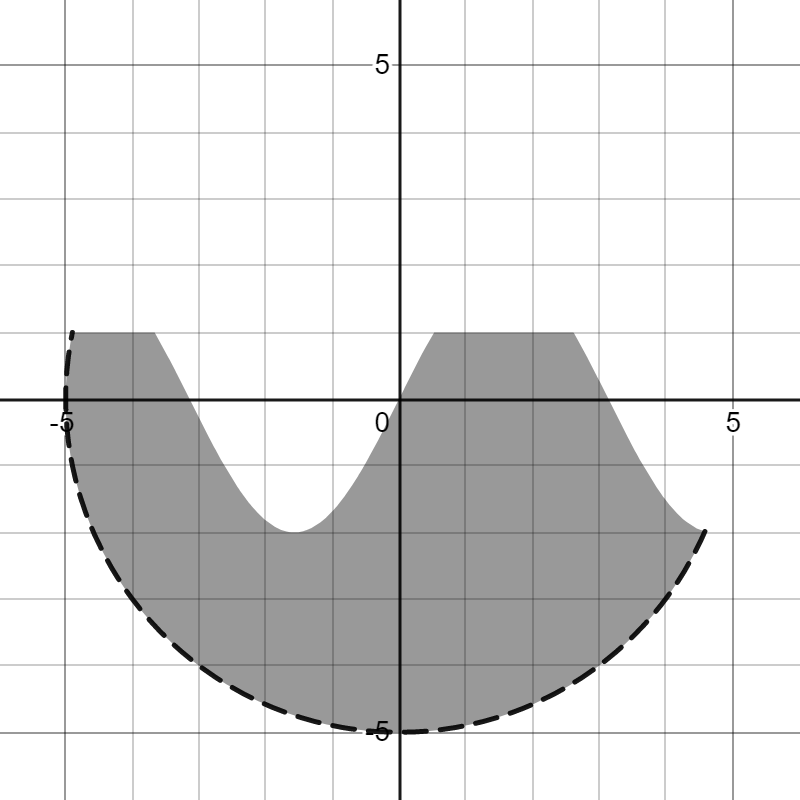
\includegraphics[width=.33\linewidth]{pic.png}}
		\caption{График неравенства}
		\label{fig:graph}
	\end{figure}

	На рисунке (\ref{fig:graph}) что-то изображено.
\end{document}